\section{Validação}

\begin{enumerate}
\item 
\end{enumerate}

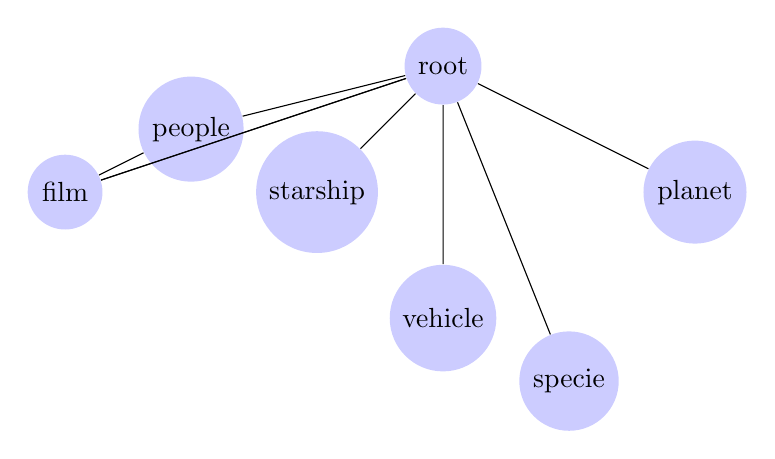
\begin{tikzpicture}
  [scale=.8,auto=left,every node/.style={circle,fill=blue!20}]
  \node (n1) at (6,10) {root};
  \node (n2) at (0,8)  {film};
  \node (n3) at (2,9)  {people};
  \node (n4) at (4,8) {starship};
  \node (n5) at (6,6)  {vehicle};
  \node (n6) at (8,5)  {specie};
  \node (n7) at (10,8)  {planet};

  \foreach \from/\to in {n1/n2,n1/n2,n1/n3,n1/n4,n1/n5,n1/n6,n1/n7,n2/n3}
    \draw (\from) -- (\to);

\end{tikzpicture}

% Servidor => Cliente
% Mudança no fluxo de dados da API

% ## Context

% - SWAPI
%   - Entities
%     - Films
%     - People
%     - Starships
%     - Vehicles
%     - Species
%     - Planets

% ## Queries

% - Gostaria de saber o nome do filme com maior numero de personagens de planeta com clima deserto
%   - Subset: Film, People, Planet
%     - films: [Film]
%       - characters: [Person]
%         - homeworld: Planet
%           - climates: [String]

% {
%   allFilms {
%     films {
%       characters {
%         homeworld {
%         	climates
%         }
%       }
%     }
%   }
% }

% - Gostaria de saber qual o nome da espécie predominante dos residentes que habitam no planeta "Alderaan".
%   - Subset: Planet, People, Species

% {
%   allPlanets {
%     planets {
%       name
%     }
%   }
% }

% {
%   planet(id: $id) {
%     residents {
%       species {
%         name
%       }
%     }
%   }
% }

% - Gostaria de saber o nome do personagem que pilota mais espaçonaves e veiculos no filme "A New Hope"
%   - Subset: Film, Starship, Vehicle, People

% {
%   allFilms {
%     films {
%       name
%     }
%   }
% }

% {
%   film(id: $id) {
%     starships {
%       pilots {
%         name
%       }
%     }
%     vehicles {
%       pilots {
%         name
%       }
%     }
%   }
% }

% ## Client

% - index (w/o graphql-jay)
% - index_2 (w/ graphql-jay)

% ## Server

% - [main] swapi (REST)
%   - https://github.com/phalt/swapi
% - swapi-graphql (GraphQL)
%   - https://github.com/graphql/swapi-graphql

% ## Test Case branches

% 1) REST Data Flow changes
% 2) REST to GraphQL migration?

% - Server Changes
%   - Mudança no Fluxo de Dados (a estrutura é a mesma)
%     - rest:
%       - endpoint renamed (just keep using the same endpoint)
%       - endpoint changed (find alternate endpoint to complement)
%       - endpoint added (faster way to access data)
%       - endpoint removed (change endpoint access)
%       - versioning (manter v1, e usar v2) [uso de composição pra transicao incremental]
%       - architecture change (manter v1, e usar graphql) [uso de composição pra transicao incremental]
%     - graphql:
%       - break into smaller schemas for services

% ## Variables

% - Qualitative
% 	- foi possível retornar os dados?
% 		- sim
% 		- não
% - Quantitative
%   - impact
%     - number of affected clients (n)
% 	- response time
% 		- milliseconds (ms)
% 	- response size
% 		- kilobytes (kb)
% 	- number of requests
% 		- GET (http)
%   - client code size
%     - lines
% 	<!-- - client code added
% 		- lines (+)
% 	- client code removed
% 		- lines (-) -->
% 	- soma do tempo de processamento local
% 		- milliseconds (ms)
